\documentclass[10pt,letterpaper]{article}
\usepackage[margin=.85in]{geometry}
\usepackage[T1]{fontenc}
\usepackage{lmodern,microtype,amsmath,amssymb,amsthm,graphicx,booktabs,xcolor}
\usepackage[colorlinks=true,linkcolor=blue!45!black,urlcolor=blue!45!black,citecolor=blue!45!black]{hyperref}
\setlength{\parindent}{0pt}
\setlength{\parskip}{5pt}
\newtheorem{theorem}{Theorem}
\newcommand{\R}{\mathbb R}
\title{\vspace{-1.3em}\textbf{Treating the Tremors We Built into Robots}\\[.35em]
\large What a checked execution layer can promise}
\author{Mike Helsel\\[-.2em]\small Working draft for technical review; AI assistance disclosed}
\date{18 October 2026}
\begin{document}
\maketitle
\vspace{-.7em}
\begin{abstract}
A smooth reference, an accepted request, and a completed task are different guarantees.
We formalize part of their connection for a scalar execution layer built from an
established four-stage moving average. Lean checks a rational finite history against
jerk and acceleration limits at every future real time. A sufficient speed check
uses the cubic Bernstein coefficients on each knot cell. A finite candidate rule
preserves committed motion and can delay or reject a new execution. A commit rule
binds the certificate to the live task, retained history, and declared timing. We prove that
completed event tails can be removed without changing future motion, and that a
checker using adjacent knot cells has the same acceleration decisions. A conditional theorem carries the physical state from time zero and proves
tracking, progress, position arrival, and terminal speed and acceleration bands
for one return task under changing response and disturbance.

A predeclared numerical comparison starts three methods from the same reference
and physical state. The retained filter has about 0.40 times the squared-jerk
integral of a native planner with matched arrival, but about 2.09 times its extra
forward travel. Only the native fast method completes the tighter task. These
results support a checked-contract case study, not a new smoothing algorithm,
a general vision-language-action (VLA) remedy, or a physical robot result.
A stronger offline smooth comparator reduces FIR's jerk integral and travel,
but raises peak jerk and still misses the tighter task. These different measures
must not be collapsed into one claim of smoothness.
\end{abstract}

\section{The guarantee has three parts}
A planner requests a task goal $g$. An executor produces a reference $q$. A
controller moves the physical position $x$. Their errors satisfy
\begin{equation}\label{eq:split}
x-g=(x-q)+(q-g).
\end{equation}
A small tracking error $x-q$ can coexist with a failed task. The reference may
arrive too late, travel too far after a reversal, or continue an old goal after
rejecting a request.

\begin{figure}[ht]
\centering
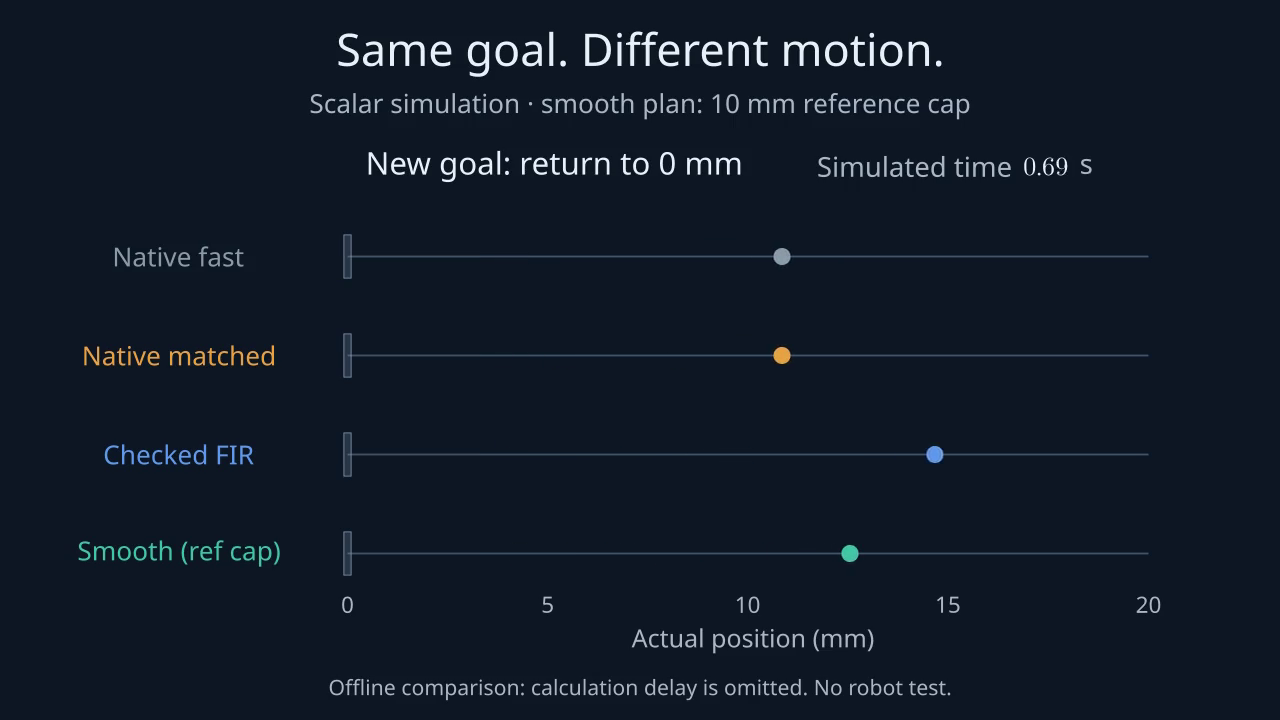
\includegraphics[width=.88\linewidth]{images/motion-animation.png}
\caption{A frame from the accompanying Manim animation. The new request is to
return to zero, but all four axes are still moving forward at the displayed
time. The paths share the same physical state at revision. This scalar
simulation uses response 100/s and zero disturbance. Planning time is omitted;
the 10 mm cap applies only to the smooth reference.}
\end{figure}

The case study asks whether a finite retained history can make these contracts
explicit and executable. It does not infer whether a new request is noise or a
real change of intent. The title describes an engineering symptom; it does not
propose a neurological mechanism.

\textbf{Prior work sets the scope.}
Finite impulse response (FIR) planning and derivative limits are established. Biagiotti and Melchiorri
already discuss acceleration growth under an overlapping reversal and waiting
as a response \cite{fir2012}. Their later work addresses time optimization under
kinematic and frequency constraints \cite{fir2019}. We use the reversal as a
regression case, not a discovery. Ruckig supplies online jerk-limited motion from
nonzero initial states \cite{ruckig}. Reference governors and ModelPlex already
connect future constraints, uncertainty, and checked execution
\cite{governors,modelplex}. A network reference governor already uses plant-side
acceptance checks for delayed or overtaken commands; its Remark 23 separates
constraint satisfaction from tracking an outdated requested reference
\cite{networkgovernor}. Timing and request identity are therefore established
design concerns. The proposed contribution is the specialized Lean
contract and its reproducible boundaries. Its research value still needs
external specialist review.

\section{Exact finite checks of a retained reference}
Let $h>0$ be one box width, and write $z_+=\max(z,0)$. The step response of four
cascaded box averages is
\[
 F(z)=\frac1{24}\sum_{k=0}^{4}(-1)^k {4\choose k}(z-k)_+^4.
\]
For a finite list of execution times and signed increments
$E=((\tau_i,\delta_i))_{i=1}^{n}$, define
\[
 q_E(t)=g_0+\sum_i\delta_i F((t-\tau_i)/h).
\]
The reference is $C^3$. Its velocity is piecewise cubic, acceleration piecewise
quadratic, and jerk piecewise affine. We call position and these first three
derivatives the reference jet. Signed cancellation remains in the
reference; we do not replace it by a sum of absolute event magnitudes.

At current time $c$, let $S$ consist of $c$ and every future knot $\tau_i+kh$,
$k=0,\ldots,4$. In each nonempty adjacent cell of $S$, add the interior zero of
jerk when jerk is nonconstant and has such a zero. Call the resulting set $C$.
When jerk is constant, acceleration is affine; its endpoints suffice. After
the final knot all derivatives vanish.

\begin{theorem}[Exact reference checks]\label{thm:checks}
For any finite event list, $h>0$, $J\geq0$, and $A\geq0$,
\[
 \bigl(\forall s\in S,\ |q_E'''(s)|\leq J\bigr)
 \ \Longleftrightarrow\
 \bigl(\forall t\geq c,\ |q_E'''(t)|\leq J\bigr),
\]
\[
 \bigl(\forall s\in C,\ |q_E''(s)|\leq A\bigr)
 \ \Longleftrightarrow\
 \bigl(\forall t\geq c,\ |q_E''(t)|\leq A\bigr).
\]
For rational inputs, the Lean Boolean checks have these all-future real
contracts. Invalid widths and negative limits are rejected.
\end{theorem}
\textit{Proof structure.} An affine function has its absolute maximum at a cell
endpoint. A quadratic function can also attain its maximum magnitude where its
derivative vanishes. The formal argument constructs cells from the event list,
including the current time and the final tail. Repeated, unsorted, expired, and
queued events are covered. It does not rely on a sampled graph.

The first acceleration implementation enumerates candidate pairs. A proved
replacement takes the minimum strictly greater knot for each left endpoint.
The theorem \texttt{same\_acceptance} equates the two Boolean results, including
invalid-input rejection. This optimization changes evaluation work, not the
accepted set.

\begin{theorem}[Removal of completed tails]\label{thm:prune}
Remove every event with $\tau_i+4h\leq c$, and add the sum of its increments to
$g_0$. For every $t\geq c$, the resulting position, velocity, acceleration, and
jerk equal those of the original reference. Both guard decisions are preserved.
\end{theorem}
Completed responses have position contribution $\delta_i$ and zero derivative.
This result does not preserve past motion or bound the number of active events.
An unbounded arrival rate can still require unbounded active history.

\textbf{A sufficient speed check.}
On a cell $[t_L,t_R]$ of length $d>0$, the cubic velocity has Bernstein
coefficients
\[
 b_0=q'(t_L),\quad b_1=q'(t_L)+\frac d3 q''(t_L),\quad
 b_2=q'(t_R)-\frac d3 q''(t_R),\quad b_3=q'(t_R).
\]
Its value is a convex combination of these four coefficients. If every
coefficient has magnitude at most $V$, the speed is at most $V$ throughout
the cell. The Lean checker connects this identity to the actual retained
reference, including its final zero-speed tail.

This is a sufficient check, unlike the exact acceleration check. A proved
example has speed at most $1/6$ but a coefficient of $3/16$, so it is rejected.
Its decision can change when the certificate partition changes, even when
the motion does not. Zero-size events can refine this speed test, but their
nominal tails also affect the timed selector. Such events are not a proved
refinement of the whole selector. The earlier pruning equivalence and timing
measurements apply to the jerk and acceleration checks, not this new guard.

\section{Admission can repair a limit and still fail a task}
A new increment is relative to the final committed target:
$\delta=g_{\mathrm{requested}}-(g_0+\sum_i\delta_i)$.
The commit rule below binds that final target to the task goal. An append-only
admission rule retains earlier events. Execution cannot precede admission.
The separately proved causal wrapper also orders execution times. Rejection
retains the existing reference. A new event contributes zero through its
execution time, so the executed position and its first three derivatives remain
unchanged.

For a finite supplied list of candidate execution times, the timed selector
checks $\tau\geq c$, speed, jerk, acceleration, and completion of every event by a
reference deadline $D$. A selected candidate therefore preserves the prefix,
meets those reference bounds, and reaches the final committed target at rest
by $D$. A result of \texttt{none} says only that all supplied certificate tests
rejected. With a conservative speed check, this does not even imply that each
listed motion violates a limit. The selector is not a complete trajectory planner.

\textbf{Fixed reversal.} Use $h=.2$ s. A $+20$ mm event starts at $.22$ s.
A return to zero becomes available at $.52$ s. An immediate $-20$ mm event
passes the jerk limit $7.5$ m/s$^3$, but its acceleration magnitude reaches
$21/32=.65625$ m/s$^2$, above the $.5$ limit. Trying execution times
$[.52,.62]$ s selects $.62$ for deadline $1.70$ s. The retained reference then
has $|q'|\leq1/15$ m/s, $|q''|\leq.5$ m/s$^2$, and $|q'''|\leq7.5$ m/s$^3$.
It reaches zero with zero derivatives at $1.42$ s. The same candidate list
returns \texttt{none} for deadline $1.30$ s.

These are exact rational Lean fixtures. They show a useful distinction:
repairing a reference limit requires time, and a deadline may not allow it.
Waiting while retaining an old motion is not an emergency stop policy.

\textbf{Bind the certificate at the future commit.}
A pending result records the exact base history, position offset, width and
version, together with the task goal, limits, request time, absolute deadline
and version. It also carries the proposed execution time and increment.
At one atomic commit, the live base and task must equal those recorded values.
Equal version integers alone are insufficient. Let $t_r,t_f,t_c,t_e$ be request,
completed computation and verification, atomic commit, and execution times.
For dispatch allowance $d\geq0$, acceptance also requires
\[
 t_r\leq t_f\leq t_c,\qquad t_c+d\leq t_e.
\]
The successful-commit theorem transfers the checked speed, acceleration, jerk
and reference-deadline conclusions to the actual appended history and live task.
It proves that the final target equals the requested goal and the old reference
jet is unchanged through execution. Rejection retains the entire live base.
Using the same certificate twice is rejected after the first commit changes
that base.

The moving fixture uses request $.52$ s, completion and commit $.57$ s,
dispatch allowance $.01$ s, and execution $.62$ s. These are exact input values
for a formal client, not measured host timing. Late completion, late commit,
changed history, changed offset, a superseded task and duplicate use are
rejected. Removing the timing check changes already executed reference position;
removing history or task binding yields a wrong final goal.

This theorem assumes one ideal clock and an atomic state check and update.
The client does not measure hardware clocks or prove a real-time implementation.
A late result can be rejected even if every result is late; rejection is not a
progress guarantee. The new rule does not make the offline optimizer causal.

\section{A conditional physical guarantee}
The scalar plant and feedback are
\begin{align}
 \dot x&=v,& \dot v&=a,& \dot a&=r(t)[u+w(t)-a],\label{eq:plant}\\
 u&=q''-8\sigma^2e_x-6\sigma e_v-\tfrac12e_a
       +\frac5{48\sigma}q''',\label{eq:feedback}
\end{align}
where $e_x=x-q$, $e_v=v-q'$, and $e_a=a-q''$. The rate satisfies
$8\sigma\leq r(t)\leq12\sigma$, and $|w(t)|\leq W$. Here $u,w,a$ have units
m/s$^2$ and $\sigma,r$ have units s$^{-1}$.

Define the transformed errors
\[
 z_1=e_x,\qquad z_2=e_x+\frac{e_v}{4\sigma},\qquad
 z_3=e_x+\frac{e_v}{2\sigma}+\frac{e_a}{16\sigma^2}.
\]
\begin{theorem}[Tracking, arrival, and a terminal hold]\label{thm:physical}
Let $H,R,W,J\geq0$ and $\sigma>0$.
Suppose a classical physical trajectory of
\eqref{eq:plant}--\eqref{eq:feedback} exists on $[0,H]$ and satisfies the stated
pointwise uncertainty bounds. If $|z_i(0)|\leq R$, $|q'''|\leq J$ on that interval,
and
\[
 W+\frac{J}{48\sigma}\leq2\sigma^2R,
\]
then $|e_x|\leq R$, $|e_v|\leq8\sigma R$, and $|e_a|\leq64\sigma^2R$ throughout it.

For the delayed-return history above, take $H\geq3.42$ s, $\sigma=10$ s$^{-1}$,
$W=.01$ m/s$^2$, $R=.2$ mm, and $J=7.5$ m/s$^3$. Under the same initial and
trajectory premises,
\[
 |x(t)-q(t)|\leq.2\ {\rm mm}\quad(0\leq t\leq H),
 \qquad x(.5)-x(0)\geq1\ {\rm mm},
\]
\[
 |x(t)|\leq.2\ {\rm mm}\quad(1.42\leq t\leq H),
\]
\[
 |v(t)|\leq.001\ {\rm m/s},\qquad |a(t)|\leq.02\ {\rm m/s^2}
 \quad(3.42\leq t\leq H).
\]
\end{theorem}
The proof derives the reference derivatives and jerk premise from the finite
history, then uses the invariant error cube. For progress,
$q(.5)=779/250000$ m and $q(0)=0$; the two position-error bounds suffice.
The sole physical initial condition is at time zero. The state is not reset
when a new request arrives.

The proof inherits the tracking cube at $t_0=1.42$ s. It shifts the same state,
response and disturbance to $t_0+s$. The zero reference tail makes the existing
feedback exactly the hold controller; no new endpoint state is supplied.

A common quadratic certificate follows the standard robust-control approach
\cite{lmibook}. On the shifted clock, let
\[
 y(s)=(80000x(t_0+s),2000v(t_0+s),50a(t_0+s)),\qquad
 E(s)=y(s)^TQ^{-1}y(s).
\]
The rational matrix
\[
 Q=\frac1{1000}\begin{bmatrix}2162&-549&-234\\-549&518&-151\\-234&-151&810\end{bmatrix}
\]
gives $\dot E\leq20(1-E)$ for every allowed response and disturbance.
Lean checks the rational matrix inequalities and their interpolation over the
response interval. The inherited cube gives $E(0)\leq10^6$, hence
\[
 E(s)\leq1+999999e^{-20s}\leq1.01\qquad(s\geq2\ {\rm s}).
\]
Its coordinate bounds give
the stated physical speed and acceleration bands. $E$ is a proof function,
not mechanical energy.

This closes the same-trajectory handoff, but its sufficient time is conservative.
The 3.42 s guarantee does not prove the numerical task at 1.70 s. The bands allow
small residual motion; they do not state exact rest. A nonzero-bias moving
witness has $x=q+12.5\,\mu$m and prevents an exact-arrival interpretation. An
independent reviewer also checked a full FIR witness with nonzero actual speed
at $3.42$ s while every theorem premise holds.
A separate exact witness rejects shifting the state while reading response and
disturbance from the old clock. No input derivative, dwell time, or constant-rate
premise is added. Existence for every bounded discontinuous input is not proved.

The parameters are illustrative, not identified from a robot. Physical
acceleration and jerk need not equal their reference limits.


\section{Comparison from the same moving state}
The experiment starts all methods from zero and uses the same FIR reference
through the left side of $.52$ s. At that revision, the common reference state is
\[
 (q,q',q'')=(77/19200,\ 23/480,\ 5/16)
\]
in SI units. The physical state is carried from time zero and is identical
across methods for each plant case.

We compare retained FIR, native fast Ruckig, and native Ruckig with minimum
duration $.90$ s. The latter matches FIR's $1.42$ s reference arrival within
the predeclared $10^{-12}$ s tolerance. The binary native duration is not an
exact rational identity. The native initial state is rounded once to binary
floating point. All methods use the same physical feedback and reference
limits $V=.1$ m/s, $A=.5$ m/s$^2$, $J=7.5$ m/s$^3$.

The frozen grid has rates $80,100,120$ s$^{-1}$, disturbances $0,.01$ m/s$^2$,
three methods, two deadlines, and output intervals $1$ and $.5$ ms:
72 traces. A full task requires request acceptance, initial progress,
reference conformity, tracking, and all three physical terminal bands from
the deadline through $2.5$ s:
\[
 |x|\leq.2\ {\rm mm},\quad |v|\leq.001\ {\rm m/s},\quad
 |a|\leq.02\ {\rm m/s^2}.
\]
A rejected revision fails the task even if the later position happens to be
near zero. Numerical terminal checks include event sides but are not an
all-time proof.

\begin{center}\small
\begin{tabular}{lrrr}
\toprule
Fine-grid results, six plant cases & Retained FIR & Native fast & Native matched\\
\midrule
Full task, deadline $1.70$ s & 6/6 & 6/6 & 6/6\\
Full task, deadline $1.30$ s & 0/6 & 6/6 & 0/6\\
$\int_{.52}^{2.5}(\dot a)^2\,dt$ (m$^2$/s$^5$)
 & 6.067--6.121 & 17.307--17.494 & 15.171--15.250\\
Extra forward excursion (mm)
 & 14.315--14.331 & 6.851--6.872 & 6.851--6.872\\
Suffix path length (mm)
 & 32.650--32.669 & 17.734--17.763 & 17.723--17.770\\
Command total variation (m/s$^2$)
 & 1.973--1.978 & 2.771--2.881 & 2.610--2.780\\
\bottomrule
\end{tabular}
\end{center}
Motion-quality ranges use the generous task over $[.52,2.5]$ s. Extra forward
excursion is measured beyond the physical position at revision, not beyond
the final target. The squared-jerk integral is a smoothness proxy, not motor
energy. Command variation includes jumps. Numerical integrals use composite
trapezoid quadrature. The two output grids are a resolution check, not a
rigorous integration error bound. Native jerk uses one-sided values at switches;
those numerical paths are not silently covered by the classical FIR theorem.

An independent replay used 80-digit arithmetic and a different physical
propagator. It checked all 271,884 state rows and 1,356 event rows with no
task-decision mismatch. Fresh native plans and 7,922 native queries matched
the saved exports. Both output grids give the same decisions. The largest
position difference between propagators was $4.2\times10^{-16}$ m. This is
agreement between numerical models, not a hardware error bar.

\begin{figure}[ht]
\centering
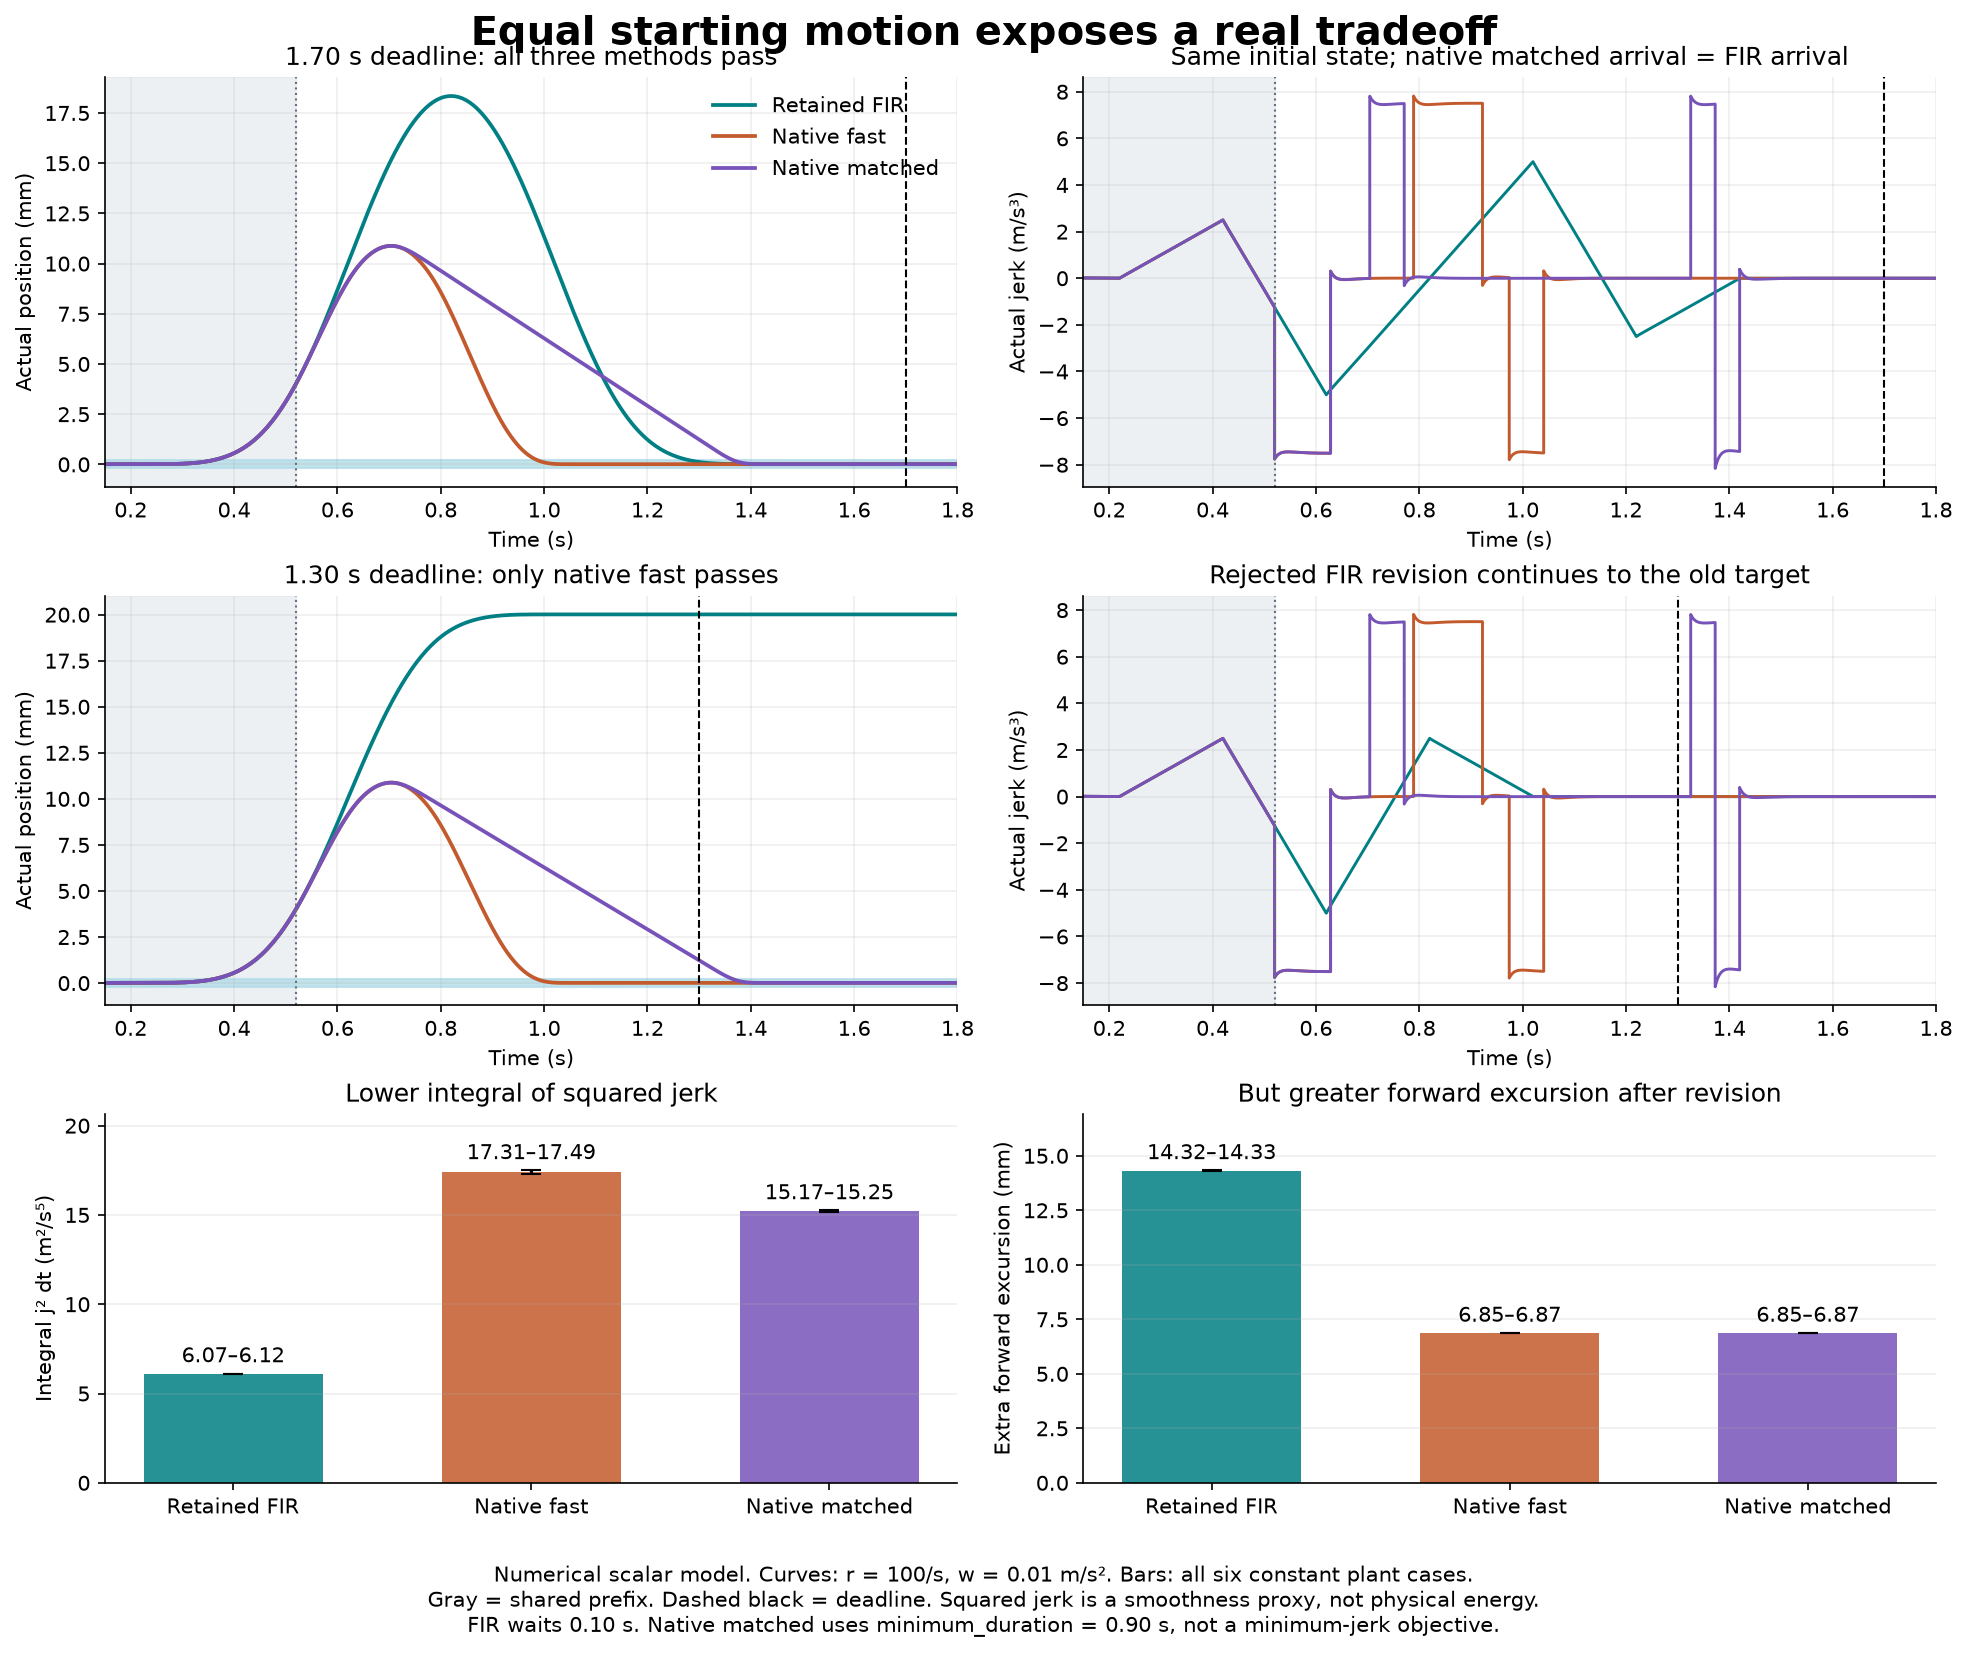
\includegraphics[width=\linewidth]{images/common-prefix.png}
\caption{The accepted common-prefix comparison shows both smoothness and travel.
Curves use the plant case stated in the figure. Both bar metrics use
$[.52,2.5]$ s. The left integrates squared jerk; the right reports maximum
extra forward excursion. Ranges cover all six declared scalar plant cases.}
\end{figure}

The FIR/native-matched squared-jerk ratio is $.398$--$.402$, while the
forward-excursion ratio is $2.085$--$2.090$. Native fast alone passes the tight
task. Matching arrival removes one confound; it does not match the paths or
make the native method a squared-jerk optimizer. We tested that remaining question with a stronger smooth baseline,
using the same arrival and an explicit reference-excursion cap.

\textbf{A stronger offline comparator.}
A convex program proposes piecewise linear jerk over the same $.90$ s suffix.
It minimizes the reference squared-jerk integral. Initial jerk is retained and
terminal jerk is zero. The reference is $C^3$; snap is not bounded.
The experiment uses CVXPY 1.9.3 with Clarabel 0.11.1
\cite{cvxpy,clarabel}. The six declared attempts use 90 or 180 intervals and forward-reference caps
of 7, 10 or 15 mm. The procedure accepts only an \texttt{optimal} solver status
followed by an exact rational reconstruction and sufficient Bernstein checks.

Only the 90-interval, 10 mm attempt passes this procedure. Two attempts return
\texttt{infeasible}; three return \texttt{optimal\_inaccurate}. None of these
statuses is used as an exact infeasibility proof. The three inaccurate attempts'
raw candidate arrays and residuals were not saved; their statuses and warnings
remain. No solve was repeated. No reference-grid convergence or optimality is
claimed. The exact repaired candidate reaches $q=q'=q''=q'''=0$ at $1.42$ s.

\begin{center}\small
\begin{tabular}{lrr}
\toprule
Six generous-task cases & Checked FIR & Smooth 10 mm reference cap\\
\midrule
Squared-jerk integral (m$^2$/s$^5$) & 6.067--6.121 & 3.692--3.766\\
Extra actual forward travel (mm) & 14.315--14.331 & 9.996--10.003\\
Peak actual jerk (m/s$^3$) & 5.000--5.002 & 7.059--8.091\\
Full task, deadline $1.70$ s & 6/6 & 6/6\\
Full task, deadline $1.30$ s & 0/6 & 0/6\\
\bottomrule
\end{tabular}
\end{center}
All 90 traces, including rejected-plan fallback, were independently replayed:
363,564 state rows and 3,294 event records. The exact polynomial checks and
numerical replay are separate evidence. The strict 10 mm reference cap does
not become a physical cap: actual travel reaches about 10.0033 mm.
The smooth candidate has a lower integral and less travel than FIR, but higher
peak jerk. Native methods still use less travel. No method dominates all
declared measures.

\begin{figure}[ht]
\centering
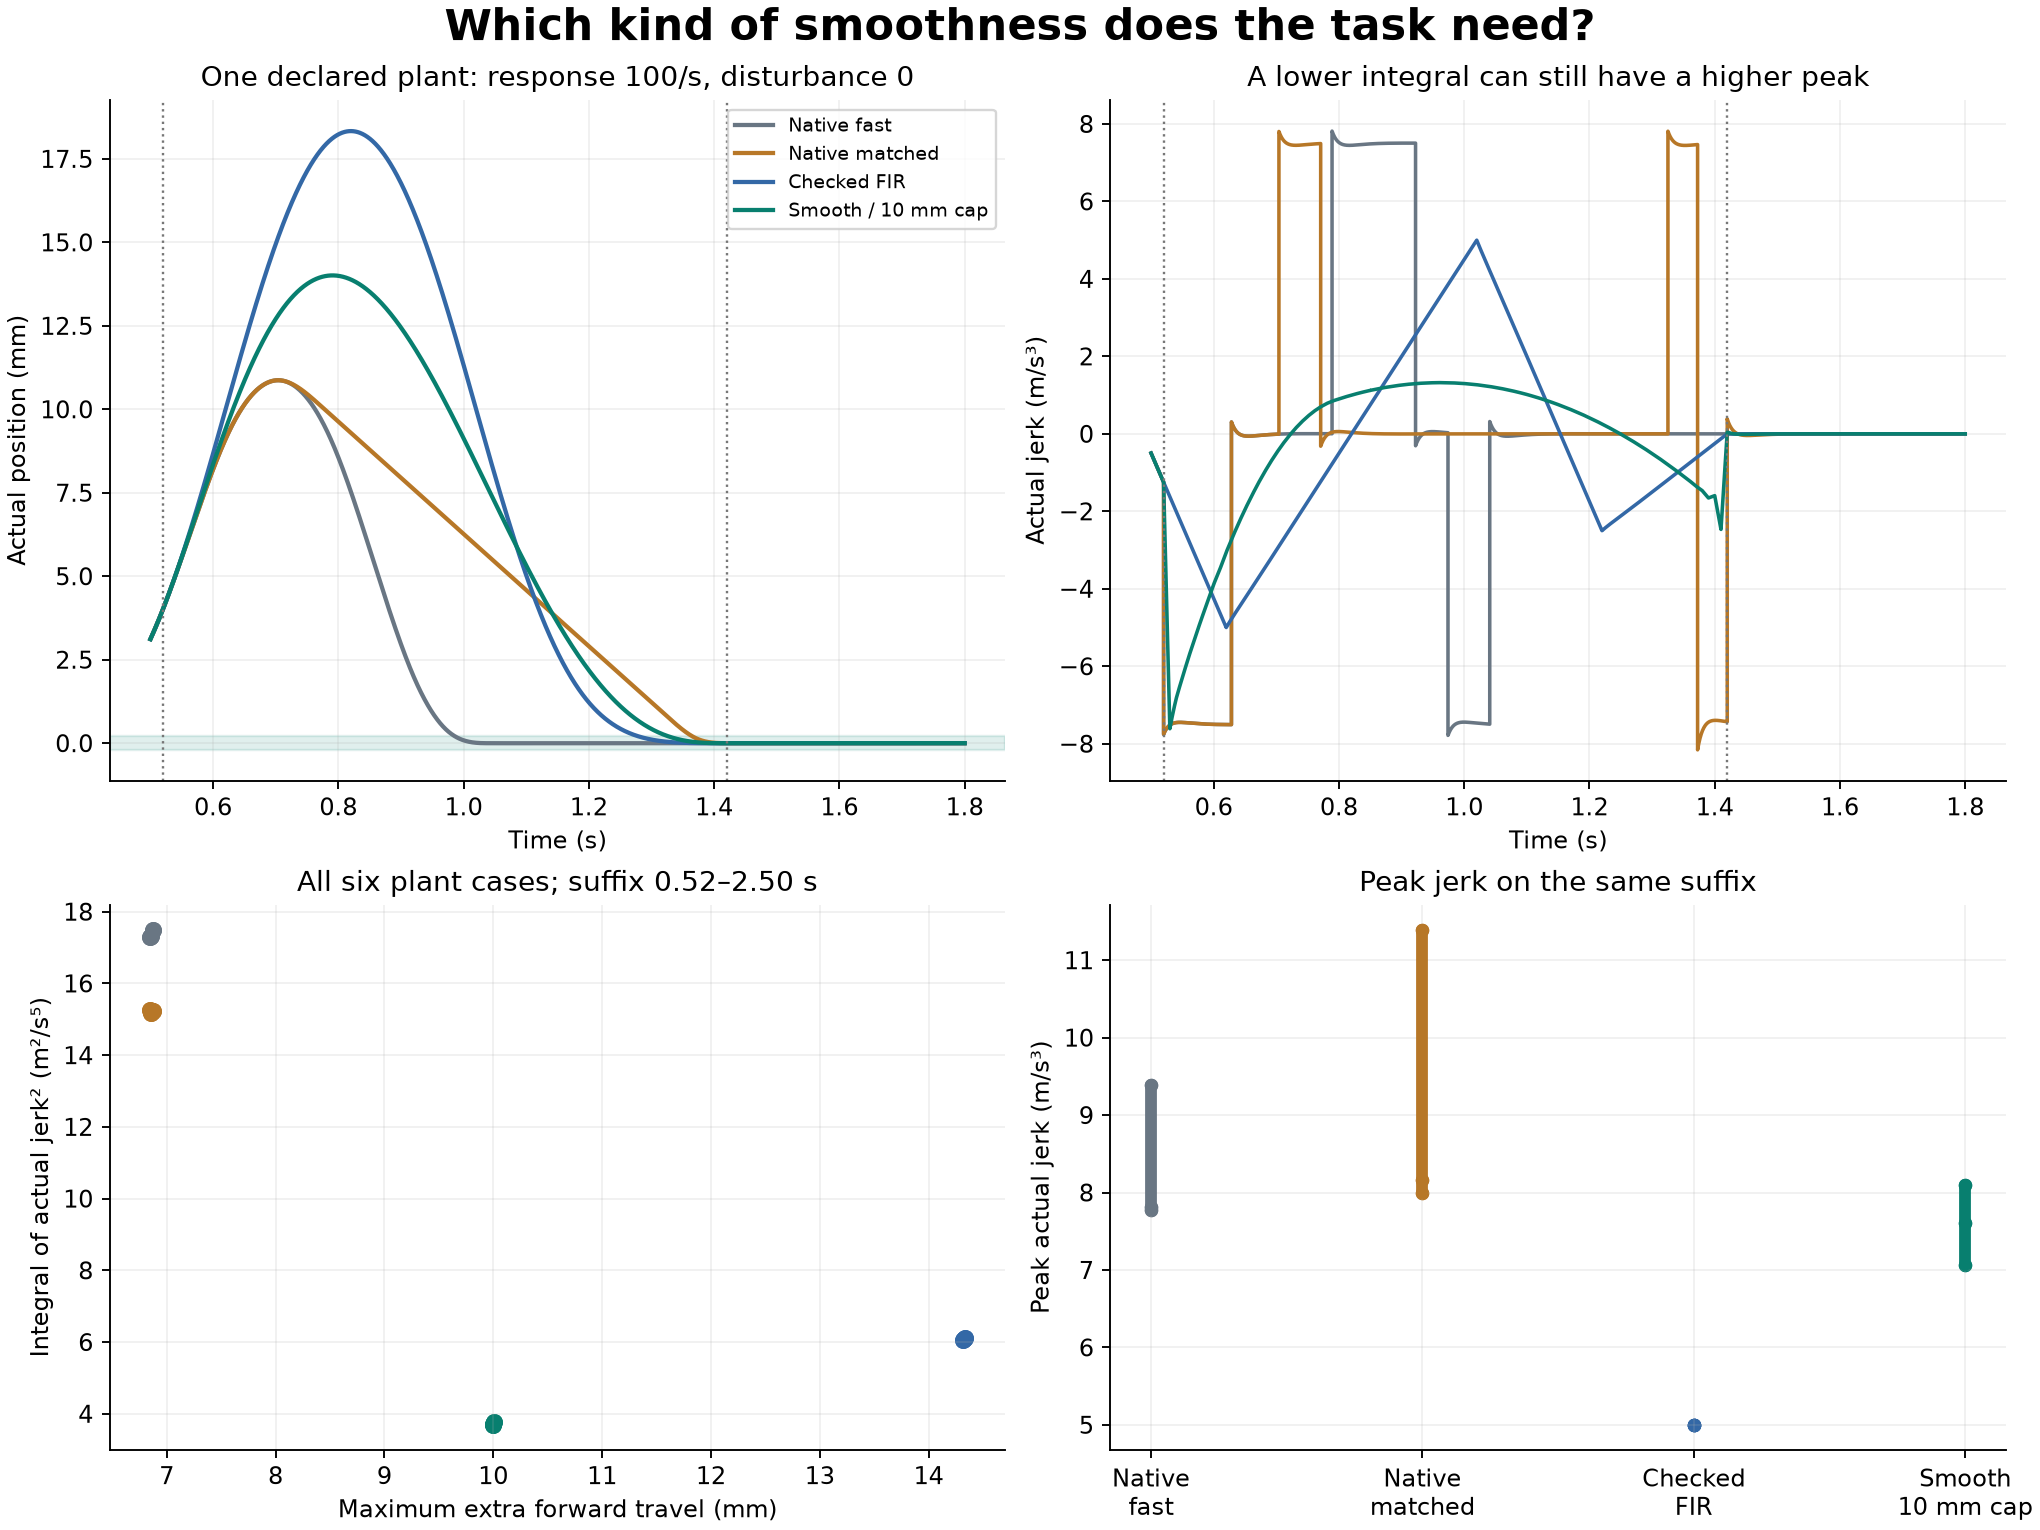
\includegraphics[width=\linewidth]{images/smooth-comparison.png}
\caption{Offline comparison from the same moving state. The 10 mm cap constrains
the reference, not actual motion. Dotted times mark $.52$ s and $1.42$ s.
Top panels show rate 100/s and zero disturbance; lower panels show the six
generous-task cases. Rejected attempts remain in the solver-outcome record.
Lower squared-jerk integral can coexist with a higher jerk peak.}
\end{figure}

\textbf{Planning latency is a separate contract.}
This comparison idealizes planning latency. The accepted solver attempt took
about $.138$ s on the recorded host, but its simulated reference begins at
$.52$ s, when the request becomes available. This is an offline matched-boundary
comparison, not demonstrated real-time replanning. A causal executor must retain
the old motion during computation, initialize a candidate at its future start,
and reject a result that is late or based on a stale plan. We have not shifted
the saved curve afterwards to hide that obligation.

\section{Proof artifact and practical limits}
The expanded portable package binds 63 local source modules to six independently
reviewed proof components. Its replay builds local sources into an empty directory,
checks every local declaration for unsafe code and unapproved axioms, separately
checks 22 module kernels, and requires 33 false clients to fail for mathematical
reasons. The replay fixes the source, reviewer, root, kernel and negative-test
plans. Public dependency caches remain a declared trust boundary. The permitted
axioms are \texttt{propext}, \texttt{Classical.choice}, and \texttt{Quot.sound}.
An independent copied-path replay passed the same source, declaration, kernel
and false-claim checks.

An offline client reads an exact rational JSON request. It saves the input bytes,
emits Lean literals, proposes a Boolean result by evaluation, then proves that
result and its consequence. Acceptance yields the reference contract; rejection
yields only unchanged live state. A separate kernel check follows. The parser,
truthful timing inputs and atomic runtime state are outside the proof. An earlier
client could report a changed input file's hash after proving its old contents.
The replacement records the digest of the parsed bytes and rejects a saved
input copy that changes during verification. Fresh output files remain trusted
local evidence, not authenticated attestation. The portable artifact records
the separate input-tool integration review.

\begin{center}\small
\begin{tabular}{p{.36\linewidth}p{.56\linewidth}}
\toprule
Paper claim & Lean entry point\\
\midrule
Exact future jerk & \texttt{check\_real\_iff}\\
Exact future acceleration & \texttt{checkAcceleration\_real\_iff}\\
Same successor acceptance & \texttt{SuccessorCheck.same\_acceptance}\\
Remove completed tails & \texttt{HistoryPruning.future\_jet\_eq}\\
Sufficient future speed & \texttt{checkVelocity\_real\_sound}\\
Timed candidate with speed & \texttt{chosen\_velocity\_reference\_contract}\\
Bound future commit & \texttt{successful\_commit\_contract}\\
Position and terminal task from initial state & \texttt{FIRHold.delayed\_return\_physical\_terminal}\\
\bottomrule
\end{tabular}
\end{center}

Exploratory shared-host timings put the new 32-event checker near 220 ms,
versus about 22.5 s for the earlier enumerating check on the same fixed inputs.
These are Lean \texttt{--run} measurements, not worst-case bounds or production
native timings. They do not establish a 1 kHz implementation. Removing completed
tails helps storage only when active event arrivals are also controlled.

The next practical test needs measured clocks, an execution schedule, a command
interface, and a coupled robot model. Franka is the intended later platform;
no robot was used here. Contact, payload variation, joint coupling, actuator
saturation, and sampled actuation need their own assumptions and acceptance
tests. The result does not certify a machine-safety performance level.

\textbf{Relation to learned and industrial execution.}
Real-Time Chunking and VLA-RAIL already retain or combine actions across changing
plans \cite{rtc,rail}. The present scalar history is not a full action chunk.
Industrial systems also expose path and timing choices: FANUC documents timing
configuration, while Yaskawa describes its SMOOTH function \cite{fanuc,yaskawa}. Those public interfaces
motivate explicit execution contracts. They do not establish the vendors'
internal algorithms or provide a measured baseline in this study.

\textbf{Review status and authorship.}
The proof gates and numerical comparison have independent agent checks.
No external human review, physical validation, public release, or paper
submission has occurred. Mike Helsel set the research question, proposed the
execution-layer direction, identified the timing interpretation, and required
fair comparisons and independent challenge. Codex agents assisted with source
review, mathematics, Lean code, numerical code, critique, figures, and writing.
Affiliation, release scope, license, and venue remain owner decisions.

\begin{thebibliography}{12}\small\raggedright
\bibitem{fir2012} L. Biagiotti and C. Melchiorri.
FIR Filters for Online Trajectory Planning with Time- and Frequency-Domain
Specifications. \emph{Control Engineering Practice} 20(12), 1385--1399, 2012.
\url{https://doi.org/10.1016/j.conengprac.2012.08.005}.
\bibitem{fir2019} L. Biagiotti and C. Melchiorri.
Trajectory generation via FIR filters: A procedure for time-optimization under
kinematic and frequency constraints. \emph{Control Engineering Practice}
87, 43--58, 2019. \url{https://doi.org/10.1016/j.conengprac.2019.03.017}.
\bibitem{ruckig} L. Berscheid and T. Kr\"oger.
Jerk-limited Real-time Trajectory Generation with Arbitrary Target States.
RSS, 2021. \url{https://arxiv.org/abs/2105.04830v2}.
\bibitem{governors} E. Garone, S. Di Cairano, and I. Kolmanovsky.
Reference and command governors for systems with constraints: A survey on
theory and applications. \emph{Automatica} 75, 306--328, 2017.
\url{https://doi.org/10.1016/j.automatica.2016.08.013}.
\bibitem{networkgovernor} S. Di Cairano, U. V. Kalabi\'c, and I. V. Kolmanovsky.
Reference Governor for Network Control Systems Subject to Variable Time-delay.
\emph{Automatica}, 2015. Author preprint, MERL TR2015-154, Section 5,
Algorithm 1 and Remark 23.
\url{https://merl.com/publications/docs/TR2015-154.pdf}.
\bibitem{modelplex} S. Mitsch and A. Platzer.
ModelPlex: Verified Runtime Validation of Verified Cyber-Physical System Models.
Runtime Verification, 199--214, 2014.
\url{https://symbolaris.com/pub/modelplex.pdf}.
\bibitem{rtc} K. Black, M. Y. Galliker, and S. Levine.
Real-Time Execution of Action Chunking Flow Policies. NeurIPS, 2025.
\url{https://arxiv.org/abs/2506.07339v2}.
\bibitem{rail} Y. Zhao et al.
VLA-RAIL: A Real-Time Asynchronous Inference Linker for VLA Models and Robots.
2025. \url{https://arxiv.org/abs/2512.24673v1}.
\bibitem{lmibook} S. Boyd, L. El Ghaoui, E. Feron, and V. Balakrishnan.
\emph{Linear Matrix Inequalities in System and Control Theory}. SIAM, 1994.
Chapter 5. \url{https://web.stanford.edu/~boyd/lmibook/index.html}.
\bibitem{cvxpy} CVXPY authors. Solver Features. Official documentation.
\url{https://www.cvxpy.org/tutorial/solvers/index.html}.
\bibitem{clarabel} P. J. Goulart and Y. Chen.
Clarabel: An interior-point solver for conic programs with quadratic objectives.
2024. \url{https://arxiv.org/abs/2405.12762}.
\bibitem{fanuc} FANUC Corporation.
How to Configure 1kHz Mode. ROS 2 Driver Documentation v2.2.0.
\url{https://fanuc-corporation.github.io/fanuc_driver_doc/v2.2.0/docs/fanuc_driver/how_to_configure_1khz_mode.html}.
\bibitem{yaskawa} Yaskawa Motoman.
SMOOTH Function Overview. 2023.
\url{https://knowledge.motoman.com/hc/en-us/articles/16313283895191-SMOOTH-Function-Overview}.
\end{thebibliography}
\end{document}
